\documentclass[submit,techrep]{ipsj}
% \documentclass{ipsj}

\usepackage{graphicx}
\usepackage{latexsym}

\def\Underline{\setbox0\hbox\bgroup\let\\\endUnderline}
\def\endUnderline{\vphantom{y}\egroup\smash{\underline{\box0}}\\}
\def\|{\verb|}

\setcounter{巻数}{59}
\setcounter{号数}{1}
\setcounter{page}{1}

% \受付{2016}{3}{4}
% \再受付{2015}{7}{16}   %省略可能
% \再再受付{2015}{7}{20} %省略可能
% \再再受付{2015}{11}{20} %省略可能
% \採録{2016}{8}{1}

\begin{document}


\title{アプリ開発における異なる実践共同体の\\
可視化システムの開発}

\etitle{Development of visualization system of different community of practice in application development}

\paffiliate{Arcana}{株式会社スタジオ・アルカナ\\
Studio Arcana, Inc.}

\paffiliate{Meisei}{明星大学情報学研究科情報学専攻\\
Department of Computer Science, Graduate School of Systems and Information Engineering, Meisei University}

\author{遠藤 勝也}{Katsuya Endoh}{Arcana}[k.endo@s-arcana.co.jp]
\author{武富 拓也}{Takuya Taketomi}{Meisei}
\author{尼岡 利崇}{Toshitaka Amaoka}{Meisei}

\begin{abstract}
  本研究では,アプリケーション開発における異なる実践共同体の参加の過程を可視化するシステムを開発した.
著者らは過去に質的アプローチの観点から実践共同体(Community of Practice以下,CoP)の概念を用いて,異なる背景を持つプロジェクトメンバーの関係のあり方が,開発されるアプリケーションにどのような影響を及ぼすかという研究を行った.その研究結果をもとにCSCW(Computer Supported Cooperative Work)の観点から,アプリケーション開発の過程における,背景の異なるプロジェクトメンバーの関わり方を可視化するシステムの開発を行った.本システムを使用することにより,異なる背景を持つメンバーが参加するアプリ開発チームにおいて,アプリのデザインをメンバー間の関係構築のあり方からデザインを考えることを支援することを目的としている.
\end{abstract}


\begin{jkeyword}
情報処理学会論文誌ジャーナル,\LaTeX,スタイルファイル,べからず集
\end{jkeyword}

\begin{eabstract}
This document is a guide to prepare a draft for submitting to IPSJ
Journal, and the final camera-ready manuscript of a paper to appear in
IPSJ Journal, using {\LaTeX} and special style files.  Since this
document itself is produced with the style files, it will help you to
refer its source file which is distributed with the style files.
\end{eabstract}

\begin{ekeyword}
IPSJ Journal, \LaTeX, style files, ``Dos and Don'ts'' list
\end{ekeyword}

\maketitle

%1
\section{はじめに}

グローバル化のもとで社会は複雑化し,ICTの進歩はめざましく,様々な業種や分野でソフトウェア・アプリケーションがなくてはならないものとなっている.現在のソフトウェア・アプリケーション(以下,アプリ)の開発は,プログラマーのみで完結することは少なく,多様な背景を持つメンバーと協働で開発が行われる.また共同開発では様々なICTツールが導入され,アプリの開発環境それ自体も変化している.
 本研究は,過去に行った異なる背景を持つプロジェクトメンバーの関係構築のあり方が,開発されるアプリケーションのデザインにどのような影響を及ぼすかという研究の結果に基に行われたものである.過去研究の結果をもとにCSCW(Computer Supported Cooperative Work)の観点からアプリケーション開発の過程における,背景の異なるプロジェクトメンバーの関わり方を可視化するシステムの開発を行った.
 過去研究は,情報学部情報学科と人文学部国際関係学科が学部横断で行ったPBL(Project Based Learning)型授業を対象に分析が行われた.観察対象のPBL型授業のテーマは,「地域観光を促進するアプリの開発」である.


CoPとは,成員の学習の促進あるいは知識を共有・創造といったある一定のテーマや目的のもとに構築された共同体である[1].
CoPの概念を用いた研究について,学習という側面に関しての多くの研究で効果が指摘されているが,異なるCoPの関係構築のあり方と開発されるアプリへの影響と変化を扱う研究は著者が知る限り少ない.しかし,上野[2]が示すように人工物は,様々な組織間やコミュニティ間の調停,交渉の産物として形成されるなど,CoPを用いた分析は学習以外にも焦点を向ける有用性があると考えられる.
 CSCW(computer supported cooperative work)では,人工物であるテクノロジーを使用場面やコンテクストに基づいて分析する研究は行われているが,コミュニケーションとアプリ開発の過程を紐付けて分析する研究はまだ少ない.著者が過去行なってきた研究ではプロジェクトメンバーの関係構築の在り方が分業的関係か協働的関係に応じて、各プロジェクトメンバーが所有する知識や技術といったリソースがその人間関係のあり方に相応して配置され、アプリのデザインに現れることを確認した[3].
本研究が対象とするPBL型授業でのアプリ開発は,ソフトウェアの開発手法の1つであるアジャイル開発が採用されている.アジャイル開発とは機能単位の小さなサイクルで,設計・開発・テストの工程を繰り返すことにより,様々な状況の変化に対応しながら開発を進めていく手法である[参考文献].状況の変化に対応するため,日毎にdaily scrumと呼ばれる短い時間での進捗の共有と反省を行う打ち合わせの時間が設けられている.導入するアプリ開発支援ソフトウェアはdaily scrumに活用されることが想定される.具体的には下記の流れを想定している.アプリ開発支援ソフトウェアは,アプリ開発に関わるタスクがどの学部(どのCoPに属しているか)の学生によって対応されたかというTrello上のデータからメンバー間の関係をグラフ構造として可視化する.その情報をもとに,アプリ開発者はタスクの質を機能中心で考えるのではなく,プロジェクトメンバーの関係性からも把握できるようになる.結果的に,開発されるアプリの機能やUIは,技術や機能中心に決定されるのではなく,プロジェクトメンバーが持つリソースを十分に利用できるような関係性から考えられるようになることを想定している.

%2
\section{先行研究}
\label{previous-research}

人文学部国際関係学科(以下,学科)と情報学部情報学科は,目的とす る専門性や実践の違いから異なるCoPであると考えられる.研究対象のプロジェクト授業に参 加する国コミ学科の学生は英語でのプレゼンテーションが主な実践であり,情報学科の学生は プログラミングやアプリ開発が主な実践となる.  アプリ開発のプロセスにおいて,当然ながらアプリの実装が完了した後で,英語でのプレゼ ンテーションという順番になるため,両学科の学生が積極的に参加するタイミングは時期に よって齟齬がおきる.加えて,国コミ学科はアプリ開発に携わった経験があるものはまれなた め,プロジェクト前半ではアプリ開発におけるコミュニケーションは積極的に意見を出すとい うよりも,観察を主とした参加の態度になる.これはCoPでいう正当的周辺参加と言い換える ことができる.他方,情報学科は技術それ自体が主な実践のため,成果発表よりも技術のそれ 自体に価値を見出す傾向が見られる.  上記のように,両学科の学生が重きを置く実践(あるいは専門)の違いが,プロジェクトに積 極的に参加する時期のずれを生み出す.その結果,言葉の解釈の違い,プロジェクトにおける 時間感覚のずれなどのディスコミュニケーションを引き起こす.  またプロジェクトに参加する態度として,自分の専門性に関わるタスクしか関心を向けない という態度は分業的なタスクの割り振りを引き起こし,このこともまたディスコミュニケー ションを引き起こす原因となる.他方,自分の専門を超えて,両学科が一緒に作業をする時間 を設けることで,アプリ開発の過程やプレゼンテーション資料作成の過程に協働で関与する中 で,言葉の意味の交渉や目的の共有が行われ,人工物のデザインに異なる専門の知識や技術的 なリソースが影響する.これはCoPでいう布置として扱われる.上記のように分業的,あるい は協働的といった関係のあり方がそれ自体が人工物の機能やUIに影響を及ぼすのではないかと いう示唆を得ている.
3. アプリ開発支援ソフトウェアに関して  本研究が対象とする授業は,両学科が自ら主とする実践や専門を越えて協働で作業すること により,お互いの実践を融合させてプロジェクトの目的を達成するように授業構成が行われて いる.そのため,本研究で導入するアプリ開発ソフトウェアは,アプリ開発の要件から実装ま でを機能中心に組み立てるのではなく、参加者それぞれの関心やスタンスを調整しその関係の あり方そのものからデザインすることを目的として実装されている.
 アプリ開発支援ソフトウェアは,Atlassia社が提供するプロジェクトのタスク管理をするた めのオンラインツールである「Trello」と連携して開発されたものである.Trelloが提供する API(Application Programming Interface)を使用して,Trelloのタスクが持つデータを抽出 し,グラフ構造として可視化する.この可視化機能により分業的,あるいは協働的にタスクを こなしているかを確認しながら,アプリ開発を行えるような想定をしている(図1).アプリ開 発支援ソフトウェアは,CoPの概念を参考に設計されており,「正統的周辺参加」をTrelloの カードの移動,プロジェクトのタスクがどの共同体に属しいてるかをTrelloのラベル機能を用 いて表す.


\section{本システムと概念の対応関係}
\label{system-map}

本システムでは,
プロジェクトメンバーをノード,
プロジェクトメンバーが共同でタスクを行った履歴をエッジとした,
ネットワーク構造でプロジェクトメンバーの関係性を可視化している.
本システムによって可視化したプロジェクトメンバーの関係性を,
図\ref{cop-map-graph}に示す.

本システムでは,ネットワーク構造のレイアウト手法として,力学モデルを採用している.
その際に,共同作業を行った回数によってエッジの強度を変化させることで,
共同でタスクを行ったプロジェクトメンバーのノードが近くに配置されるようになっている.
% これにより,

また,プロジェクトメンバーの所属先によってノードの色を変化させることで,
異なるCoPに所属するプロジェクトメンバーの共同作業を観察することを可能にしている.
これにより,異なる色のノードがエッジでつながっている様子から,
布置を観察することを可能にしている.

さらに,タスクを行った回数の合計値によってノードの大きさを変化させる.
これにより,ノードの大きさは小さいが,他のノードとの繋がりがみられる場合に,
そのプロジェクトメンバーは正統的周辺参加であるという可能性を観察することができる.

以上のネットワーク構造を,プロジェクトの時系列順に変化させることで,
プロジェクトメンバーの関係性の変化を観察することを可能にしている.
これにより,ノードの軌跡から,
進行状況によって変化していく,
プロジェクトメンバーのトラジェクトリーを観察することを可能にしている.

% \begin{enumerate}
%    \item CoP
%    \item 布置
%    \item トラジェクトリー
%    \item 正統的周辺参加
% \end{enumerate}

\begin{figure}[h]
  \centering
  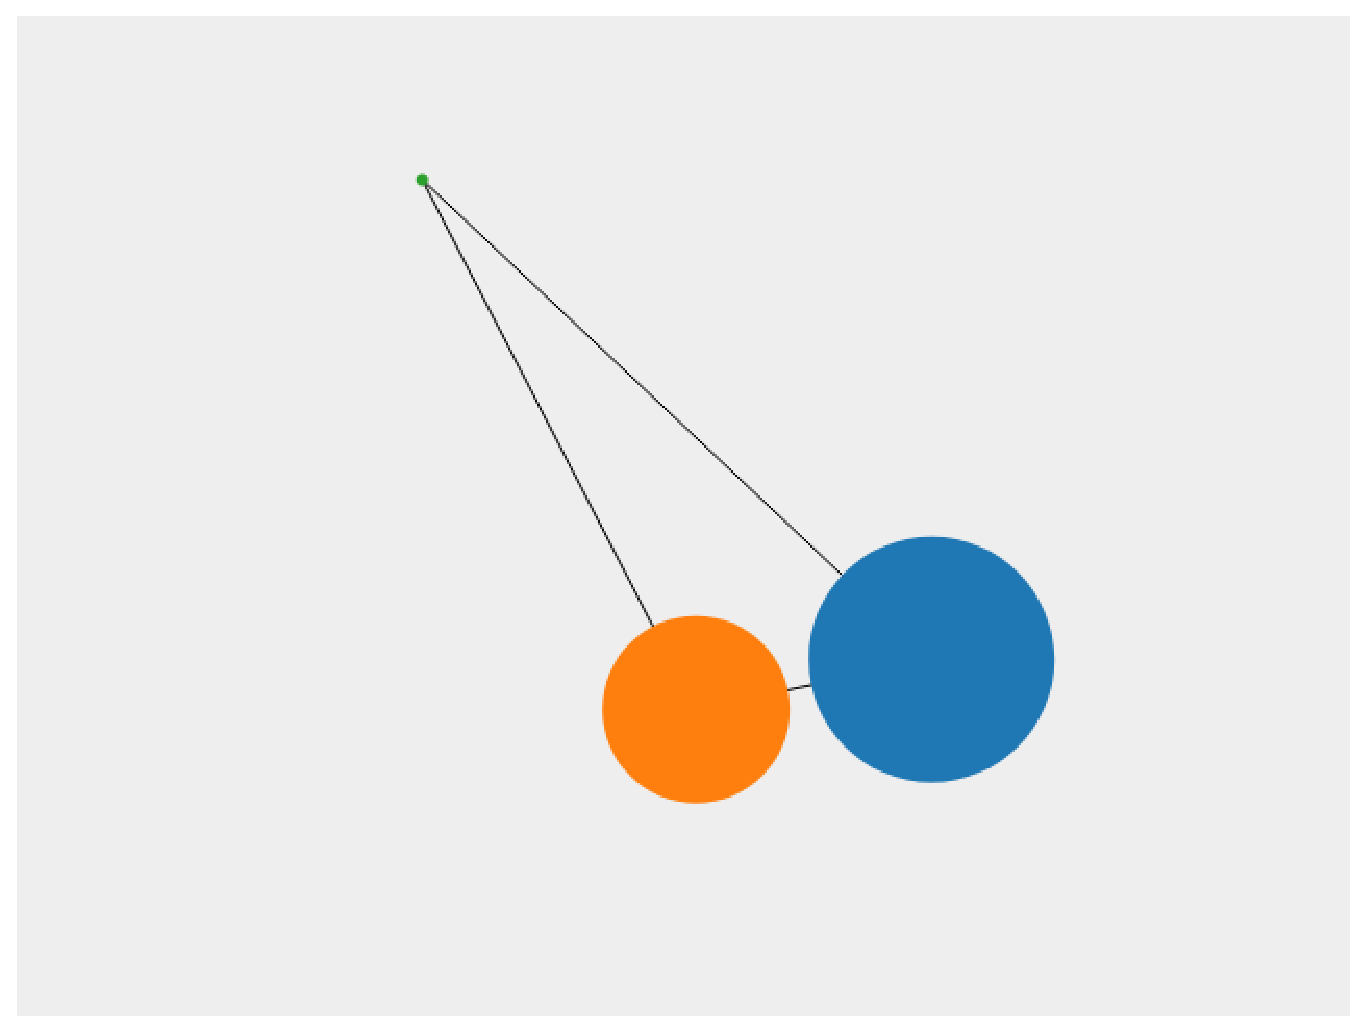
\includegraphics[width=0.5\textwidth]{img/cop-map-graph.eps}
  \caption{プロジェクトメンバーの関係性を可視化した様子}
  \label{cop-map-graph}
\end{figure}

\section{本システムの実装}
\label{implementation}

本システムは,アプリケーションサーバとデータベース,外部サービスであるTrelloから構成される.


%4
\section{今後の展望}

%5
\section{おわりに}

\begin{thebibliography}{9}
\bibitem{okumura}
奥村晴彦:改訂第5版 \LaTeXe 美文書作成入門,
技術評論社(2010).

\bibitem{companion}
Goossens, M., Mittelbach, F. and Samarin, A.: {\it The LaTeX Companion},
Addison Wesley, Reading, Massachusetts (1993).

\bibitem{book1}
木下是雄:
理科系の作文技術,
中公新書(1981).

\bibitem{book2}
Strunk, W.J. and White, E.B.: {\it The Elements of Style, Forth Edition},
Longman (2000).

\bibitem{book3}
Blake, G. and Bly, R.W.: {\it The Elements of Technical Writing},
Longman (1993).

\bibitem{book4}
Higham, N.J.:
{\it Handbook of Writing for the Mathematical Sciences},
SIAM (1998).

\bibitem{webpage1}
情報処理学会論文誌ジャーナル編集委員会:
投稿者マニュアル(オンライン),
\urlj{http://www.ipsj.or.jp/journal/ submit/manual/j\_manual.html}%
\refdatej{2007-04-05}.

\bibitem{webpage2}
情報処理学会論文誌ジャーナル編集委員会:
べからず集(オンライン),
\urlj{http://www.ipsj.or.jp/journal/\\ manual/bekarazu.html}%
\refdatej{2011-09-15}.

\end{thebibliography}

\begin{biography}
\profile{n}{遠藤 勝也}{1992年生.2016年明星大学情報学部情報学科卒業.
2018年株式会社スタジオ・アルカナ入社.ウェブサービス開発に従事.芸術科学会会員.}
%
\profile{n}{武富 拓也}{1990年生.2016年明星大学人文部国際コミュニケーション学科卒業.
2019年明星大学情報学部実習指導員として勤務, 明星大学大学院情報学研究科情報学専攻博士前期課程(研究生). 社会言語科学会会員}
%
\profile{h,L}{学会 次郎}{1950年生.1974年架空大学大学院修士課程修了.
1987年同博士課程修了.工学博士.1977年架空大学助手.1992年情報処理大学助
教授.1987年同大教授.2000年から情報処理学会顧問.オンライン出版の研究
に従事.2010年情報処理記念賞受賞.情報処理学会理事.電子情報通信学会,
IEEE,IEEE-CS,ACM 各会員.}
\end{biography}

\end{document}
